\section{多智能体协作与研究过程控制}
\subsection{角色分工与通信拓扑}
多智能体系统将复杂研究分配给可区分的任务主体，并通过消息或共享状态协调活动。
角色可以按专业知识划分，也可以按研究阶段或工具权限划分。
前者有利于跨学科问题讨论，后者便于明确交付物和验收标准。
两种划分可以结合，但角色名称本身不能解释收益：其作用需要通过获得的信息、承担的动作和对其他主体的约束来说明。

图\ref{fig:topology}归纳了三种常见组织形式。
流程型协作沿既定依赖传递结果，适合文献整理、实现与核对等顺序较清楚的任务；
中心调度型协作由协调者分配子任务和整合输出，便于管理资源及处理分支；
讨论型协作允许主体交换候选与批评，更适合尚未固定研究路径的探索。
AutoGen支持通过可编程交互构造多种模式\cite{autogen}，MetaGPT则强调标准化操作流程及中间产物\cite{metagpt}。
实际系统往往同时采用多种拓扑，不能仅凭一张角色图认定其全部控制方式。

\begin{figure*}[t]\centering
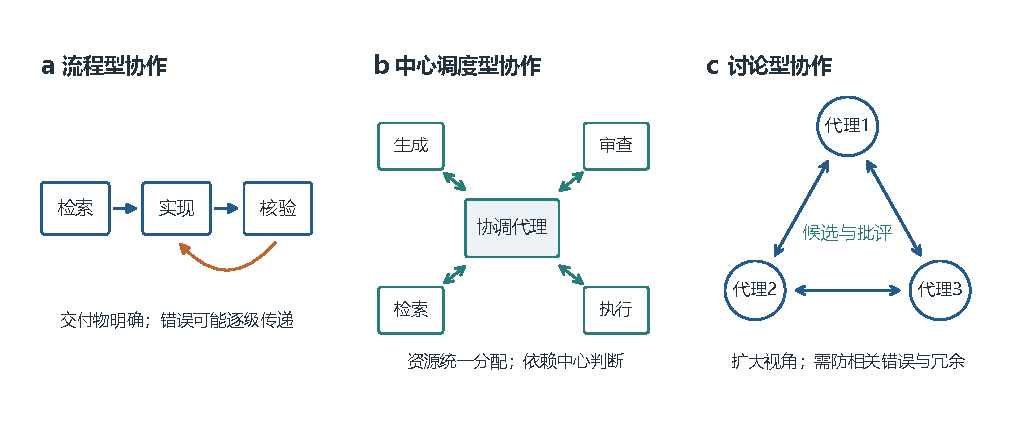
\includegraphics[width=\textwidth]{figures/review-topologies.pdf}
\caption{多智能体协作的三种基本组织形式。依据代理交互、标准化流程与多代理辩论研究归纳\cite{autogen,metagpt,debate}。
节点表示功能主体，边表示允许的交互；图示用于分析组织差异，不将某一框架限定为单一拓扑。}
\label{fig:topology}\end{figure*}

通信结构影响系统效率，也影响错误传播。
流水线可以减少无关讨论，但上游遗漏可能被下游连续接受；
中心调度便于统一判断，却形成对协调者的依赖；
自由讨论扩大了信息交换范围，也增加重复消息、状态不一致和过早形成共识的可能。
在$n$个代理每轮两两通信的理想化设置中，$T$轮对应的有向消息数为$Tn(n-1)$。
实际费用还取决于消息长度、工具调用和重试次数，但这一关系已经说明通信开销需要随协作规模一起评价。

\subsection{任务分解与标准化交付}
将研究目标拆成子任务，既是能力分配问题，也是约束传递问题。
如果任务定义只有“完成实验”或“检查结果”，后续代理仍需自行猜测哪些数据、指标和条件应被保留。
MetaGPT将标准化操作程序嵌入角色协作，使中间产物成为后续工作的共同依据\cite{metagpt}。
科研系统可以借鉴这一思路，将文献证据、实验方案、运行记录和结论依据作为不同交付对象。

标准化的作用并不是增加固定格式，而是减少信息在交接中的损失。
检索环节应说明来源支持何种判断，实验环节应保留比较条件及配置，
分析环节应区分观测结果与解释，报告环节则需要维持结论范围。
只有这些对象能够相互对应，检查者才能判断问题来自任务定义、程序实现还是结果解释。
相反，若交付仅包含经过润色的摘要，流程虽然更简洁，返工和审计却会更加困难。

任务分解还需适应研究的不确定性。
对目标明确的复现任务，固定流程通常有利于控制变量；
对假设探索任务，过早固定步骤可能限制新证据引起的方向调整。
因此，流程约束宜优先固定研究原则和交付内容，对探索路径保留一定灵活性。
这种区分能够兼顾研究过程的开放性与实验比较的可解释性。

\subsection{反馈、反思与辩论的作用条件}
ReAct将外部行动观察纳入推理过程，为科研代理调用检索和程序工具提供了基本交互模式\cite{react}。
Reflexion进一步让反馈影响后续尝试\cite{reflexion}，多代理辩论则通过交换不同回答与理由，
使系统在部分推理和事实任务中改善结果\cite{debate}。
这些工作共同说明，增加修订机会能够带来收益，但收益来源并不相同：
可能来自新证据、错误定位、候选多样性，也可能来自更多推理样本。

因此，需要区分外部反馈与语言层面的再评价。
编译器可以判断部分程序错误，测试可以检验预先规定的行为，实验仪器则提供关于物理对象的观察；
模型批评主要评价已有材料中的合理性和一致性。
它们都可能有用，但能够支持的结论范围不同。
Huang等对内在自我纠错的研究表明，没有可靠外部反馈时，所测推理任务的修订并不稳定\cite{correct}。
这与辩论方法在部分任务上的正向结果并不矛盾，因为任务、信息来源和计算设置不同。

多角色的独立性也需要具体判断。
使用相同基础模型并不必然使协作无效，但共享资料和错误前提会限制检查增量。
检索者寻找支持材料，反例搜索者专门寻找相反证据，执行者独立重算结果，
比多个角色重复评价同一段文字更容易形成互补信息。
由此可见，协作设计的重点在于构造有意义的差异，而非仅增加身份设定。

\subsection{从固定流程到搜索调度}
当研究存在多个候选方案时，协作还需要决定资源应投向哪条路径。
The AI Scientist-v2引入实验管理代理和渐进式树搜索，将候选实现、调试及改进组织为分支探索\cite{scientistv2}。
AI co-scientist则通过假设比较和演化调整候选集合\cite{cosci}。
前者的反馈更多来自可执行实验与评价，后者更侧重假设和研究建议的质量。
二者分别展示了实现空间与假设空间中的搜索控制。

搜索带来更广的探索机会，也引入候选选择偏差。
若多次尝试始终围绕测试集成绩选择方案，最终报告可能高估泛化能力；
若候选排名仅依赖同类模型判断，则可能偏好容易表述、符合常见叙事的想法。
因此，搜索效率、研究质量和评价有效性应分别报告。
对科研系统而言，保留候选淘汰原因、失败尝试和最终选择依据，
比单独展示最优分支更有助于理解其实际能力。
